\subsubsection*{Station Matching}
\label{ssub:station_matching}

  Das Station Matching war eines der fundamentalen Herausforderungen bei der Programmierung des Servers. Es ist dafür da, um die Distanz zwischen den einzelnen Stationen zu ermitteln. Zwar hat das Stuttgart-VVS Feed ein \texttt{stop\_distance\_traveled} Feld, welches die benötigten Distanz Informationen direkt aus der Datenbank liefert, aber für andere GTFS-Feeds die getestet wurden, ist dieses Feld oftmals nicht vorhanden. Die Applikation verwendet also das \texttt{stop\_distance\_traveled} Feld, falls es vorhanden ist und als Fallback-Lösung erfolgt die Berechnung via Station Matching Algorithmus.\\

  Das Station Matching soll folgendes Problem lösen:

  \begin{figure}[htbp]
    \begin{center}
      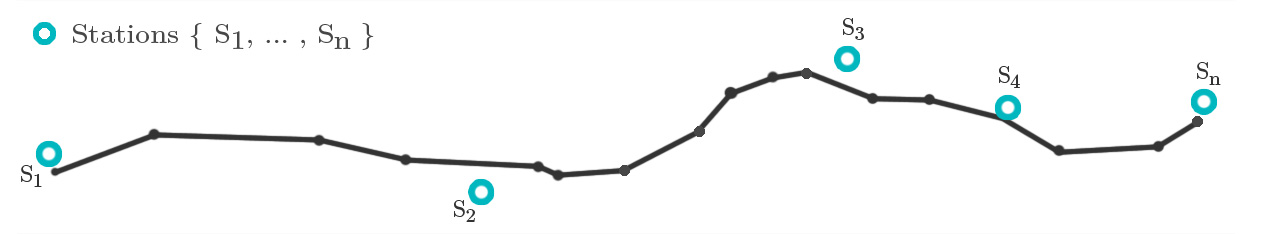
\includegraphics[width=\textwidth]{station_problem.jpg}
      \caption{Stationen liegen nicht direkt auf der Polyline}
      \label{fig:station_problem}
    \end{center}
  \end{figure}
  
  Wie in Grafik \ref{fig:station_problem} zu sehen ist liegen die Stationen nicht exakt auf der Polyline, sondern sind ein wenig abseits platziert. So entspricht die Position der Station einer Haltestelle oder Bahnhof. Meistens befinden sich diese ein wenig versetzt zum eigentlichen Verlauf der Strecke. Die Visualisierung interpoliert die Bewegung eines Vehicles zwischen den einzelnen Stationen. Damit das möglich ist, wird die zurückzulegende Distanz zwischen den einzelnen Stationen benötigt. Um sie zu berechnen ist es nötig die Stationen auf die Polyline zu legen (das Matching).

  \begin{figure}[htbp]
    \begin{center}
      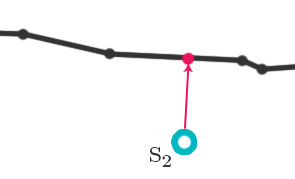
\includegraphics[width=0.25\textwidth]{find_nearest_point}
      \caption{Finde den am nächstgelegenen Punkt der Station auf der Polyline}
      \label{fig:find_nearest_point}
    \end{center}
  \end{figure}

  Nachdem ein Punkt auf der Polyline gefunden ist, kann die Distanz berechnet werden. Die Distanzen zweier Stationen $\{s_i,s_{i+1} \;|\; i \in \mathbb{N} \}$ sei $d_\triangle$. Diese kann jetzt wie folgt berechnet werden: $ d_\triangle = d_{i+1} - d_i$. 

  \begin{figure}[htbp]
    \begin{center}
      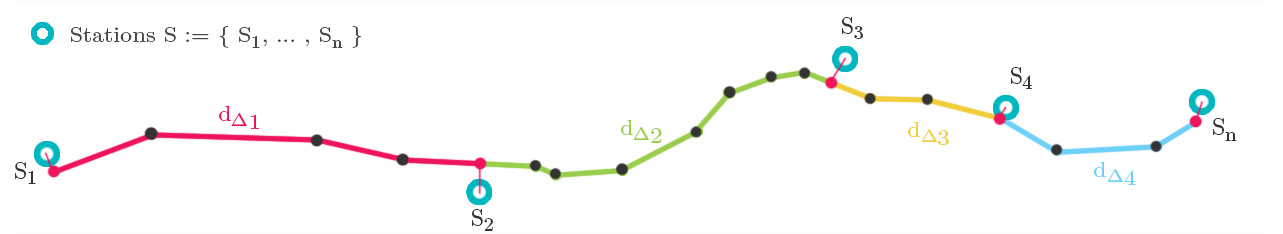
\includegraphics[width=\textwidth]{get_distances}
      \caption{Berechnen der Distanz}
      \label{fig:get_distances}
    \end{center}
  \end{figure}
  
  In Listing \ref{lst:match_station} des Anhangs wird ein Algorithmus vorgestellt, der das Problem des Station Matchings und der Distanzberechnung löst. Abbildung \ref{fig:station_matching_comparision} stellt eine frühere Implementierung mit der nun aktuellen Version des Algorithmus gegenüber. Dafür wird Zeit, die der jeweilige Algorithmus zum Matching über $n$-Trips benötigt verglichen. Um eine durchschnittliche Laufzeit zu erhalten wurde jeder Algorithmus 10 mal mit der gleichen Anzahl an Trips ausgeführt.

  \begin{figure}[htbp]
    \begin{center}
      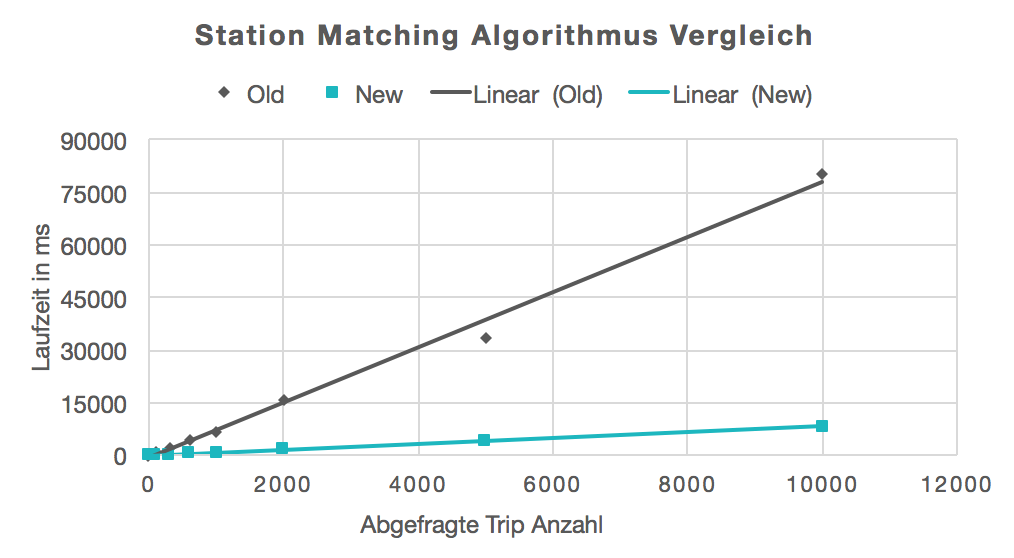
\includegraphics[width=0.7\textwidth]{station_matching_comparision}
      \caption{Vergleich der zwei Station Matching Algorithmen}
      \label{fig:station_matching_comparision}
    \end{center}
  \end{figure}

  Der alte Algorithmus war sehr simpel und beruhte darauf die Funktion \texttt{pointOnLine} der \texttt{Turf.js} Bibliothek zu verwenden. Diese Funktion hatte den entscheidenden Nachteil, dass sie in 3 \texttt{for}-Schleifen über die gesamten Punkte der Polyline iteriert. Hinzu kommt, dass das Matching nicht nur auf eine Station, sondern auf sämtliche Stationen aus allen Trips angewendet werden muss. Das führte dazu, dass insgesamt 5 \texttt{for}-Schleifen verwendet wurden. Damit lässt sich der im Vergleich höhere Anstieg der Laufzeit bei steigender Trip Anzahl erklären.

  Generell ist der neue Algorithmus sehr viel schneller. Durch die Verwendung eines \texttt{R-Trees}\footnotemark und der eigenen Implementierung verschiedener Bibliotheksfunktionen, konnte die Laufzeit drastisch reduziert werden (siehe Tabelle \ref{tbl:station_matching_comparison}). 

  \begin{longtable}{|>{\raggedright \arraybackslash}p{5.0cm}|>{\raggedright \arraybackslash}p{5.0cm}|>{\raggedright \arraybackslash}p{5.0cm}|}
  \caption{Station Matching Vergleich Old / New}\label{tbl:station_matching_comparison}\\
    \hline
    Anz. verarbeiteter Trips & Old (in ms)& New (in ms)\\
    \hline
    100    & 712   & 121  \\
    300    & 2191  & 305  \\
    600    & 4344  & 545  \\
    1.000  & 6780  & 874  \\
    2.000  & 15782 & 1700 \\
    5.000  & 33708 & 4161 \\
    10.000 & 80291 & 8279 \\
    \hline
  \end{longtable}

  Zwar wachsen beide Implementierungen lediglich Linear mit steigender Trip Anzahl, allerdings benötigt der neue Algorithmus für die Verarbeitung von $10.000$ Tausend Trips anstatt $80.29$ nur $8.28$ Sekunden.  

  Im Realbetrieb verarbeitet der Server zwischen $0 - 500$ Trips. Bei dieser Anzahl beträgt die Laufzeit des Algorithmus $\approx80ms - 400ms$. Dadurch kann argumentiert werden, dass der Algorithmus gerade noch schnell genug für eine Webanwendung arbeitet. Auch größere Anzahlen an Trips wären noch in akzeptabler Geschwindigkeit berechenbar. So können $1000$ Trips immer noch in unter einer Sekunde berechnet werden. Allerdings wäre es bei einer größeren Anzahl an Trips, der falsche Ansatz diese bei jeder Serveranfrage zu kalkulieren. Besser wäre es, einmalig das Matching für alle Trips eines GTFS Feeds durchzuführen und die Ergebnisse persistent in der Datenbank abzuspeichern. Dies könnte beispielsweise gleich beim Importieren der Daten in die Datenbank geschehen. Dadurch kann die Berechnung komplett eingespart werden. Da für das Stuttgart-VVS Feed glücklicherweise die zurückgelegte Distanz bis zu einer Station, bereits zur Verfügung steht, muss nur noch die Distanz zwischen den Stationen ($d\triangle$) berechnet werden. Dies geschieht nach dem selben Prinzip wie in der oben genannten Formel: $ d_\triangle = d_{i+1} - d_i$. Diese Berechnung ist trivial und erfolgt bei $10.000$ Trips in unter 15 Millisekunden.

  \footnotetext{Ein R-Tree (R für Rectangle) bezeichnet eine Baumförmige Datenstruktur für das Speichern und Abfragen von raumbezogenen Informationen. In Verwendung ist folgende Bibliothek: \url{https://github.com/mourner/rbush}}
  
% subsubsection station_matching (end)